%% Version 4.3.2, 25 August 2014
%
%%%%%%%%%%%%%%%%%%%%%%%%%%%%%%%%%%%%%%%%%%%%%%%%%%%%%%%%%%%%%%%%%%%%%%
% Template.tex --  LaTeX-based template for submissions to the 
% American Meteorological Society
%
% Template developed by Amy Hendrickson, 2013, TeXnology Inc., 
% amyh@texnology.com, http://www.texnology.com
% following earlier work by Brian Papa, American Meteorological Society
%
% Email questions to latex@ametsoc.org.
%
%%%%%%%%%%%%%%%%%%%%%%%%%%%%%%%%%%%%%%%%%%%%%%%%%%%%%%%%%%%%%%%%%%%%%
%  PREAMBLE
%%%%%%%%%%%%%%%%%%%%%%%%%%%%%%%%%%%%%%%%%%%%%%%%%%%%%%%%%%%%%%%%%%%%%

%% Start with one of the following:
%  DOUBLE-SPACED VERSION FOR SUBMISSION TO THE AMS
%\documentclass{ametsoc}

%  TWO-COLUMN JOURNAL PAGE LAYOUT---FOR AUTHOR USE ONLY
\documentclass[twocol]{ametsoc}

\usepackage{multirow}
\usepackage{gensymb}

%%%%%%%%%%%%%%%%%%%%%%%%%%%%%%%%
%%% To be entered only if twocol option is used

\journal{jcli}

%  Please choose a journal abbreviation to use above from the following list:
% 
%   jamc     (Journal of Applied Meteorology and Climatology)
%   jtech     (Journal of Atmospheric and Oceanic Technology)
%   jhm      (Journal of Hydrometeorology)
%   jpo     (Journal of Physical Oceanography)
%   jas      (Journal of Atmospheric Sciences)	
%   jcli      (Journal of Climate)
%   mwr      (Monthly Weather Review)
%   wcas      (Weather, Climate, and Society)
%   waf       (Weather and Forecasting)
%   bams (Bulletin of the American Meteorological Society)
%   ei    (Earth Interactions)

%%%%%%%%%%%%%%%%%%%%%%%%%%%%%%%%
%Citations should be of the form ``author year''  not ``author, year''
\bibpunct{(}{)}{;}{a}{}{,}

%%%%%%%%%%%%%%%%%%%%%%%%%%%%%%%%

%%% To be entered by author:

%% May use \\ to break lines in title:

\title{Comparison of present reanalysis datasets in the context of the analogue method for statistical precipitation downscaling.}

%%% Enter authors' names, as you see in this example:
%%% Use \correspondingauthor{} and \thanks{Current Affiliation:...}
%%% immediately following the appropriate author.
%%%
%%% Note that the \correspondingauthor{} command is NECESSARY.
%%% The \thanks{} commands are OPTIONAL.

    %\authors{Author One\correspondingauthor{Author One, 
    % American Meteorological Society, 
    % 45 Beacon St., Boston, MA 02108.}
% and Author Two\thanks{Current affiliation: American Meteorological Society, 
    % 45 Beacon St., Boston, MA 02108.}}

\authors{Pascal Horton\correspondingauthor{University of Bern, Institute of Geography, Hallerstrasse 12, 3012 Bern, Switzerland.}, Rolf Weingartner, Stefan Br\"{o}nnimann}

%% Follow this form:
    % \affiliation{American Meteorological Society, 
    % Boston, Massachusetts.}

\affiliation{Oeschger Centre for Climate Change Research, Institute of Geography, University of Bern, Bern, Switzerland}

%% Follow this form:
    %\email{latex@ametsoc.org}

\email{pascal.horton@giub.unibe.ch}

%% If appropriate, add additional authors, different affiliations:
    %\extraauthor{Extra Author}
    %\extraaffil{Affiliation, City, State/Province, Country}

\extraauthor{Charles Obled}
\extraaffil{Laboratoire d'\'{e}tude des Transferts en Hydrologie et Environnement (LTHE), Universit\'{e} de Grenoble-Alpes, Grenoble, France}


%%%%%%%%%%%%%%%%%%%%%%%%%%%%%%%%%%%%%%%%%%%%%%%%%%%%%%%%%%%%%%%%%%%%%
%  ABSTRACT
%
% Enter your abstract here
% Abstracts should not exceed 250 words in length!
%
% For BAMS authors only: If your article requires a Capsule Summary, please place the capsule text at the end of your abstract
% and identify it as the capsule. Example: This is the end of the abstract. (Capsule Summary) This is the capsule summary. 

\abstract{The analogue method is a statistical downscaling method for precipitation prediction. It uses similarity in terms of synoptic-scale predictors with situations in the past in order to provide a probabilistic prediction for the day of interest. It has been used for decades in a context of weather or flood forecasting, and is more recently also applied to climate studies, whether for reconstruction of past weather conditions or future climate impact studies. In order to evaluate the relationship between synoptic scale predictors and the local weather variable of interest, e.g. precipitation, reanalysis datasets are necessary. Nowadays, the number of available reanalysis datasets increase. These are generated by different atmospheric models with different assimilation techniques and offer various spatial and temporal resolutions. A major difference between these datasets is also the length of the archive they provide. While some datasets start at the beginning of the satellite era and assimilate these data, others aim at homogeneity on a longer period and only assimilate conventional observations.
The context of the application of analogue methods might drive the choice of an appropriate dataset, for example when the archive length is a leading criterion. However, in many studies, a reanalysis dataset is subjectively chosen, according to the user’s preferences or the ease of access. The impact of this choice on the results of the downscaling procedure is rarely considered and no comprehensive comparison has been undertaken so far.
In order to fill this gap and to advise on the choice of appropriate datasets, nine different global reanalysis datasets were compared in seven distinct versions of analogue methods, over 300 precipitation stations in Switzerland. Significant differences in terms of prediction performance were identified. Although the impact of the reanalysis dataset on the skill score varies according to the chosen predictor, be it atmospheric circulation or thermodynamic variables, some hierarchy between the datasets is often preserved.
}

\begin{document}

%% Necessary!
\maketitle


%%%%%%%%%%%%%%%%%%%%%%%%%%%%%%%%%%%%%%%%%%%%%%%%%%%%%%%%%%%%%%%%%%%%%
%  MAIN BODY OF PAPER
%%%%%%%%%%%%%%%%%%%%%%%%%%%%%%%%%%%%%%%%%%%%%%%%%%%%%%%%%%%%%%%%%%%%%
%

%% In all cases, if there is only one entry of this type within
%% the higher level heading, use the star form: 
%%
% \section{Section title}
% \subsection*{subsection}
% text...
% \section{Section title}

%vs

% \section{Section title}
% \subsection{subsection one}
% text...
% \subsection{subsection two}
% \section{Section title}

%%%
% \section{First primary heading}

% \subsection{First secondary heading}

% \subsubsection{First tertiary heading}

% \paragraph{First quaternary heading}


%TODO: publish results as datasets?

\section{Introduction}

\section{Data and methods}

\subsection{Reanalysis datasets}

\cite{Compo2011}

\cite{Kanamitsu2002}


\subsection{Precipitation dataset}


\subsection{Considered analogue methods}




%TODO: rewrite
Multiple variations of the analogue method exist, most of which are not detailed here \cite[see][for a more comprehensive listing]{BenDaoud2016}. However, there are mainly two parameterizations that are most often used for precipitation prediction and that are considered as reference: one that relies on an analogy of the atmospheric circulation, and another that adds a second level of analogy on moisture variables \citep{Obled2002, Bontron2005, Marty2012}.

The method based on the analogy of synoptic circulation consists of the following steps (Table \ref{table:params_R1}): the similarity of the atmospheric circulation of a target date with every day of the archive is assessed by processing the S1 criterion \citep[Eq.\ \ref{eq:S1}, ][]{Teweles1954, Drosdowsky2003}, which is a comparison of gradients, over a certain spatial window:

\begin{equation}
\label{eq:S1}
S1=100 \frac {\displaystyle \sum_{i} \vert \Delta\hat{z}_{i} - \Delta z_{i} \vert}
{\displaystyle \sum_{i} max\left\lbrace \vert \Delta\hat{z}_{i} \vert , \vert \Delta z_{i} \vert \right\rbrace }
\end{equation}
where $\Delta \hat{z}_{i}$ is the difference in geopotential height between the \textit{i}-th pair of adjacent points of gridded data describing the target situation, and $\Delta z_{i}$ is the corresponding observed geopotential height difference in the candidate situation. The differences are processed separately in both North and East directions over the selected spatial domain. The smaller the S1 values, the more similar the pressure fields.

\citet{Bontron2005} showed that the geopotential height at 500~hPa (Z500) and 1000~hPa (Z1000) are the best first predictors of the NCEP/NCAR reanalysis I dataset, and that the S1 criterion performs better than scores based on absolute distances. The reason for such better results is that the S1 criterion allows comparison of the circulation patterns, by means of the gradients, rather than the absolute value of the geopotential height, which better represent the flow direction. To cope with seasonal effects, candidate dates are extracted within a period of four months centred around the target date, for every year of the archive. This method using two geopotential heights is named here 2Z.

The $N_{1}$ dates with the lowest values of S1 are considered as analogues to the target day. The number of analogues, $N_{1}$, is a parameter to calibrate. Then, the daily observed precipitation amount for the $N_{1}$ selected dates provide the empirical conditional distribution, considered as the probabilistic prediction for the target day.

The other most well-known parametrization adds a second level of analogy on the moisture variables (method 2Z-2MI, Table \ref{table:params_R2}). The predictor that \citet{Bontron2004} found optimal for France is a moisture index made of the product of the total precipitable water (TPW) with the relative humidity at 850~hPa (RH850). \cite{Horton2012a} confirmed that this index is also better for the Swiss Alps than any other variable from the NCEP/NCAR reanalysis I considered independently. When adding a second level of analogy, $N_{2}$ dates are subsampled within the $N_{1}$ analogues of the atmospheric circulation, to end up with a smaller number of analogue situations. When this second level of analogy is added, a higher number of analogues $N_{1}$ is kept on the first level. Prediction of moisture fields by NWP models are more model-dependent and more uncertain than pressure variables. This implies that the 2Z-2MI method, when used in real-time forecasting, is very dependent on the skill of the NWP model in predicting moisture fields. Therefore its use is often restricted to the first lead times.


%TODO: not sensitive to biases

\subsection{Performance assessment}



%TODO: rewrite
The performance assessment in the present context consists of verifying the prediction of an ensemble probabilistic technique. The set of precipitation values collected with each analogue can be considered as a sample drawn from the conditional distribution associated with the current circulation. The score that is most often used to assess an AM performance is the CRPS \citep[Continuous Ranked Probability Score,][]{Brown1974, Matheson1976, Hersbach2000}. It allows evaluating the predicted cumulative distribution functions $F(y)$, for example, of the precipitation values $y$ from analogue situations, compared to the observed value $y^{0}$. The better the prediction, the smaller the score. The mean CRPS of a prediction series of length $n$ can be written as:

\begin{equation}
\label{eq:CRPS}
CRPS = \frac{1}{n} \sum_{i=1}^{n} \left(  \int_{-\infty}^{+\infty} \left[ F_{i}(y)-H_{i}(y-y_{i}^{0})\right]^{2} dy \right) 
\end{equation}
where $H(y-y_{i}^{0})$ is the Heaviside function that is null when $y-y_{i}^{0}<0$, and has the value 1 otherwise.

In order to compare the value of the score relative to a reference, one often considers its skill score expression, and uses the climatological distribution of precipitation from the entire archive as the reference. The CRPSS (Continuous Ranked Probability Skill Score) is thus defined as follows:

\begin{equation}
\label{eq:CRPSS}
CRPSS = \frac{CRPS-CRPS_{r}}{CRPS_{p}-CRPS_{r}} = 1-\frac{CRPS}{CRPS_{r}}
\end{equation}
where $CRPS_{r}$ is the CRPS value for the reference and $CRPS_{p}$ would be the one for a perfect prediction (which implies $CRPS_{p}~=~0$). A better prediction is characterized by an increase in CRPSS.

Note, however, that the choice of reference does not matter so much when assessing potential improvements of the method, since we consider more its relative increase or decrease rather than the CRPSS absolute value.



\section{Influence of the reanalysis dataset}

\subsection{Mean performance}

\subsection{Precipitation occurrence}

\subsection{High precipitation events}

\subsection{Selection of the analogue dates}


\section{Further analyzes}

\subsection{Influence of the spatial resolution}

\subsection{Archive length vs ensembles}

\subsection{On the spread of the ensemble in early years}

%TODO: 20CR spread decrease with time -> low for present & high in the past


\subsection{Precipitation data from the reanalysis}


\section{Discussion}


\section{Conclusion}


%%%%%%%%%%%%%%%%%%%%%%%%%%%%%%%%%%%%%%%%%%%%%%%%%%%%%%%%%%%%%%%%%%%%%
%  ACKNOWLEDGMENTS
%%%%%%%%%%%%%%%%%%%%%%%%%%%%%%%%%%%%%%%%%%%%%%%%%%%%%%%%%%%%%%%%%%%%%
%
\acknowledgments
Start acknowledgments here.

%%%%%%%%%%%%%%%%%%%%%%%%%%%%%%%%%%%%%%%%%%%%%%%%%%%%%%%%%%%%%%%%%%%%%
%  APPENDIXES
%%%%%%%%%%%%%%%%%%%%%%%%%%%%%%%%%%%%%%%%%%%%%%%%%%%%%%%%%%%%%%%%%%%%%
%
% Use \appendix if there is only one appendix.
%\appendix

% Use \appendix[A], \appendix}[B], if you have multiple appendixes.
%\appendix[A]

%% Appendix title is necessary! For appendix title:
%\appendixtitle{}

%%% Appendix section numbering (note, skip \section and begin with \subsection)
% \subsection{First primary heading}

% \subsubsection{First secondary heading}

% \paragraph{First tertiary heading}

%% Important!
%\appendcaption{<appendix letter and number>}{<caption>} 
%must be used for figures and tables in appendixes, e.g.,
%
%\begin{figure}
%\noindent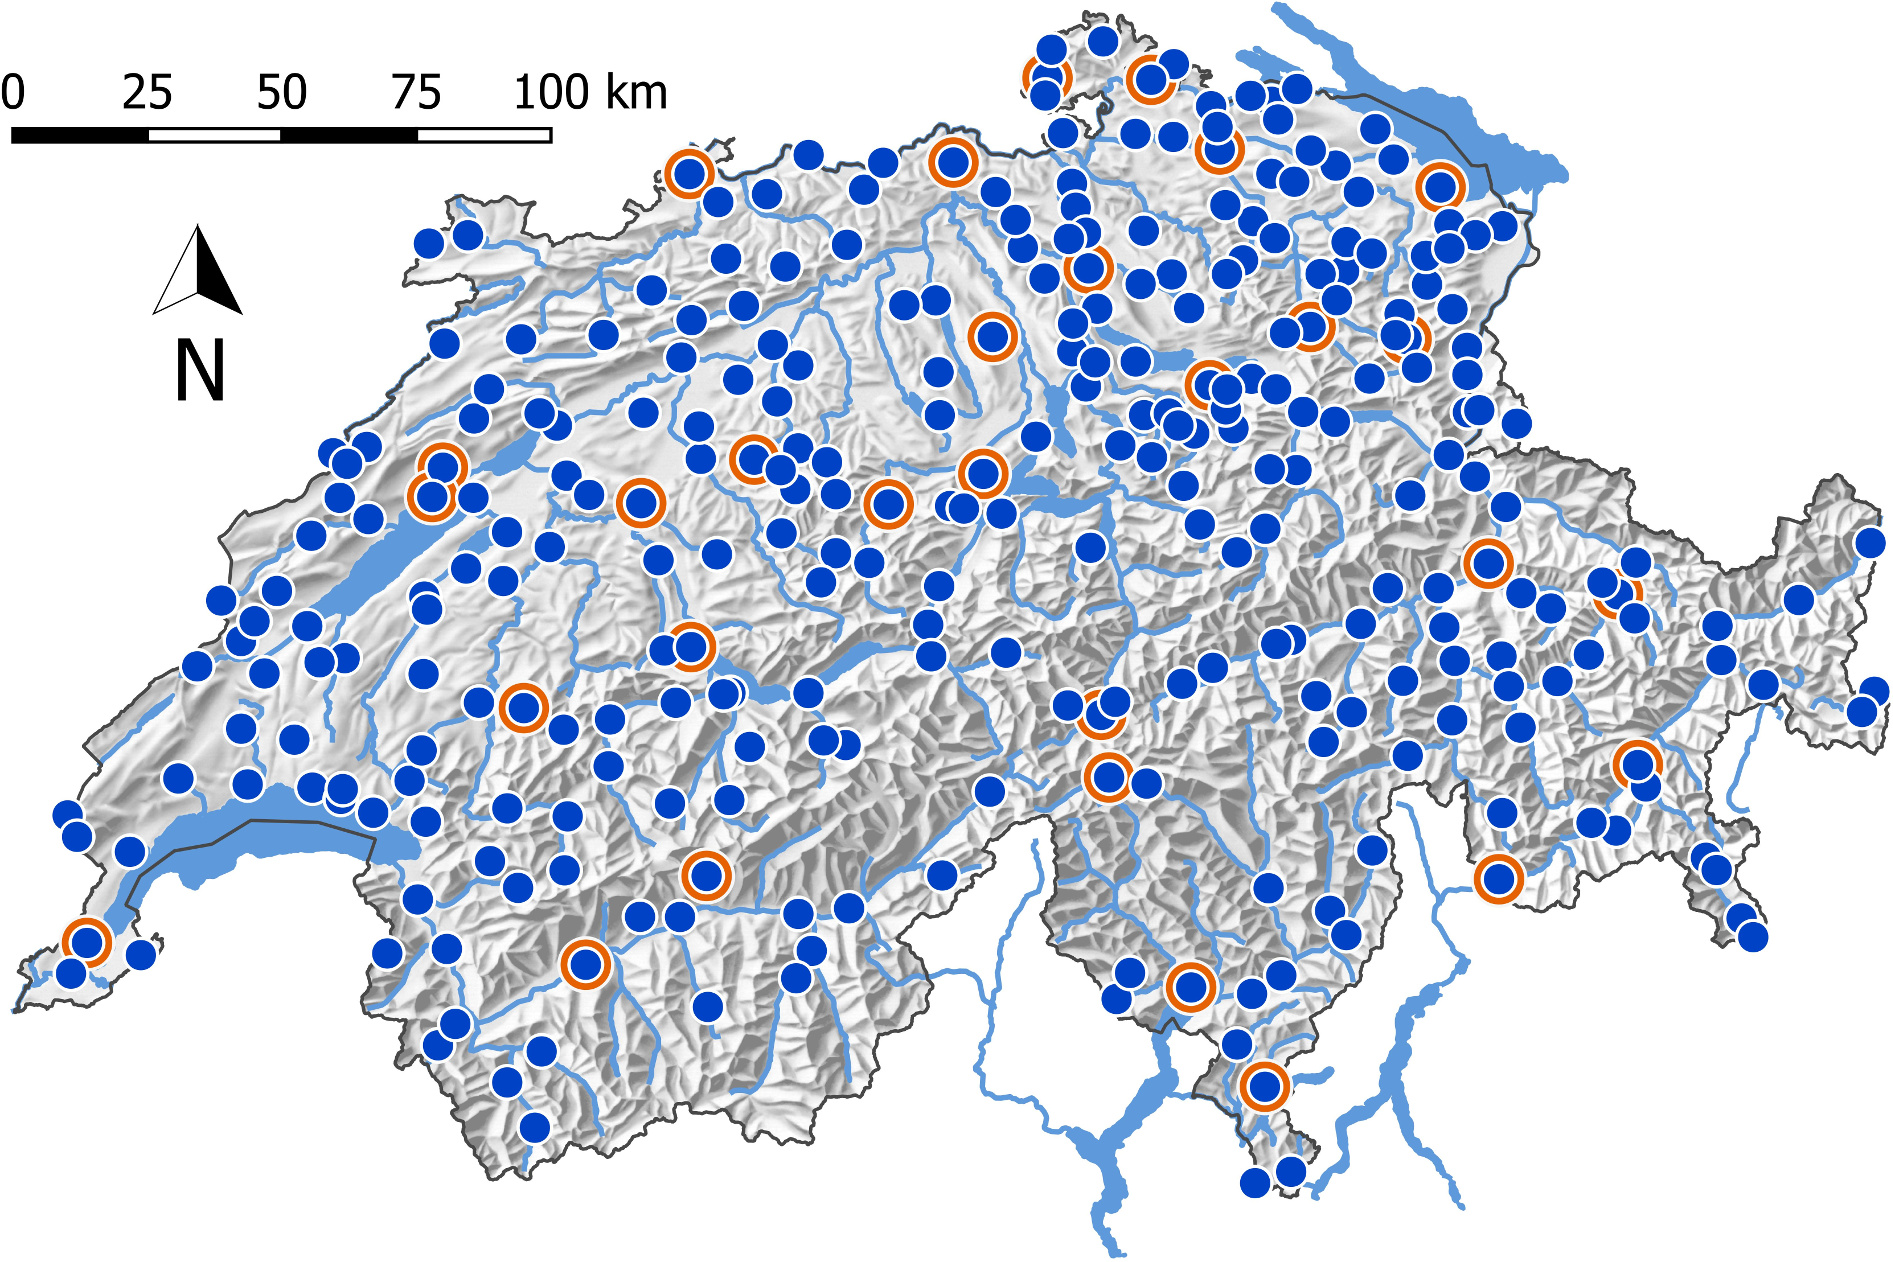
\includegraphics[width=19pc,angle=0]{figure01.pdf}\\
%\appendcaption{A1}{Caption here.}
%\end{figure}
%
% All appendix figures/tables should be placed in order AFTER the main figures/tables, i.e., tables, appendix tables, figures, appendix figures.
%
%%%%%%%%%%%%%%%%%%%%%%%%%%%%%%%%%%%%%%%%%%%%%%%%%%%%%%%%%%%%%%%%%%%%%
%  REFERENCES
%%%%%%%%%%%%%%%%%%%%%%%%%%%%%%%%%%%%%%%%%%%%%%%%%%%%%%%%%%%%%%%%%%%%%
% Make your BibTeX bibliography by using these commands:
\bibliographystyle{ametsoc2014}
\bibliography{../../../Biblio/Mendeley/Export/4_articles-2017_JCli_reanalysis}


%%%%%%%%%%%%%%%%%%%%%%%%%%%%%%%%%%%%%%%%%%%%%%%%%%%%%%%%%%%%%%%%%%%%%
%  TABLES
%%%%%%%%%%%%%%%%%%%%%%%%%%%%%%%%%%%%%%%%%%%%%%%%%%%%%%%%%%%%%%%%%%%%%
%% Enter tables at the end of the document, before figures.
%%
%
%\begin{table}[t]
%\caption{This is a sample table caption and table layout.  Enter as many tables as
%  necessary at the end of your manuscript. Table from Lorenz (1963).}\label{t1}
%\begin{center}
%\begin{tabular}{ccccrrcrc}
%\hline\hline
%$N$ & $X$ & $Y$ & $Z$\\
%\hline
% 0000 & 0000 & 0010 & 0000 \\
% 0005 & 0004 & 0012 & 0000 \\
% 0010 & 0009 & 0020 & 0000 \\
% 0015 & 0016 & 0036 & 0002 \\
% 0020 & 0030 & 0066 & 0007 \\
% 0025 & 0054 & 0115 & 0024 \\
%\hline
%\end{tabular}
%\end{center}
%\end{table}


\begin{table*}[t]
	\caption{Considered analogue methods with increasing complexity. P0 is the preselection (PC: on calendar basis, that is $\pm 60$ days around the target date), L1, L2 and L3 are the subsequent levels of analogy. The meteorological variables are: SLP -- mean sea level pressure, Z -- geopotential height, T -- air temperature, W -- vertical velocity, MI -- moisture index, which is the product of the relative humidity at the given pressure level and the total water column. The analogy criterion is S1 for SLP and Z and RMSE for the other variables.}
	\begin{center}
		\begin{tabular}{cccccl}
			\hline
			\textbf{Method} & \textbf{P0} & \textbf{L1} & \textbf{L2} & \textbf{L3} & \textbf{Reference} \\ 
			\hline 
			\multirow{2}{*}{\textbf{2SLP}} & \multirow{2}{*}{PC} & SLP@12h &&& \\
			&& SLP@24h &&& \\
			\hline 
			\multirow{2}{*}{\textbf{2Z}} & \multirow{2}{*}{PC} & Z1000@12h &&& \multirow{2}{*}{\citealt{Bontron2004}} \\
			 && Z500@24h &&& \\
	 		\hline 
			\multirow{4}{*}{\textbf{4Z}} & \multirow{4}{*}{PC} & Z1000@06h &&& \multirow{4}{*}{\citealt{Horton2017b}} \\
			 && Z1000@30h &&& \\
			 && Z700@24h &&& \\
			 && Z500@12h &&& \\
			\hline 
			\multirow{2}{*}{\textbf{2Z-2MI}} & \multirow{2}{*}{PC} & Z1000@12h & \multirow{2}{*}{MI850@12+24h} && \multirow{2}{*}{\citealt{Bontron2004}} \\
			&& Z500@24h &&& \\
			\hline 
			\multirow{4}{*}{\textbf{4Z-2MI}} & \multirow{4}{*}{PC} & Z1000@30h &&& \multirow{4}{*}{\citealt{Horton2017b}}\\
			&& Z850@12h & MI700@24h && \\
			&& Z700@24h & MI600@12h && \\
			&& Z400@12h &&& \\
			\hline 
			\multirow{2}{*}{\textbf{PT-2Z-4MI}} & T925@36h & Z1000@12h & MI925@12+24h && \multirow{2}{*}{\citealt{BenDaoud2016}} \\
			& T600@12h & Z500@24h & MI700@12+24h && \\
			\hline 
			\multirow{2}{*}{\textbf{PT-2Z-4W-4MI}} & T925@36h & Z1000@12h & \multirow{2}{*}{W850@06-24h} & MI925@12+24h & \multirow{2}{*}{\citealt{BenDaoud2016}} \\
			& T600@12h & Z500@24h && MI700@12+24h & \\
			\hline 
			
		\end{tabular} 
	\end{center}
	\label{table:methods}
\end{table*}



\begin{table*}[t]
	\caption{Assessed reanalysis datasets with their respective available period, timestep and resolution.}
	\begin{center}
		\begin{tabular}{ccccccc}
			\hline
			\multirow{2}{*}{\textbf{Id}} & \multirow{2}{*}{\textbf{Institutions}} & \multirow{2}{*}{\textbf{Name}} & \textbf{Period} & \textbf{Output} & \textbf{Model} & \multirow{2}{*}{\textbf{Assimilation}}\\ 
			&&& \textbf{of record} & \textbf{resolution} & \textbf{vintage} &\\ 
			\hline 
			\textbf{NNR-1} & NCEP, NCAR & Reanalysis I & 1948/01 -- present & 2.5\degree x 2.5\degree & 1995 & 3D-Var\\
			\textbf{NDR-2} & NCEP, DOE & Reanalysis II & 1948/01 -- present & 2.5\degree x 2.5\degree & 2001 & 3D-Var\\
			\textbf{ERA-INT} & ECMWF & ERA-Interim & 1979/01 -- present & 0.75\degree x 0.75\degree & 2006 & 4D-Var\\
			\textbf{CFSR} & NCEP & Clim. Forecast Sys. Rean. & 1979/01 -- present & 0.5\degree x 0.5\degree & 2009 & 3D-Var\\
			\textbf{JRA-55}  & JMA & Japanese 55-year Rean. & 1957/12 -- 2016/01 & 1.25\degree x 1.25\degree & 2009 & 4D-Var\\
			\textbf{JRA-55C}  & JMA & JRA-55 Conventional Data & 1957/12 -- 2016/01 & 1.25\degree x 1.25\degree & 2009 & 4D-Var\\
			\textbf{20CR-2c} & NOAA-CIRES & 20th Century Rean. V2c & 1850/12 -- 2014/12 & 2\degree x 2\degree & 2009 & E. K. filter\\
			\textbf{ERA-20C} & ECMWF & ERA 20th century & 1900/01 -- 2011/01 & 1\degree x 1\degree & 2012 & 4D-Var\\
			\textbf{MERRA-2} & NASA & MERRA-2 & 1980/01 -- present & 0.625\degree x 0.5\degree & 2014 & 3D-Var\\
			\textbf{CERA-20C} & ECMWF & CERA-20C & 1901/01 -- 2010/12 & 1\degree x 1\degree & 2016 & 4D-Var\\
			\hline 
		\end{tabular} 
	\end{center}
	\label{table:datasets}
\end{table*}







%%%%%%%%%%%%%%%%%%%%%%%%%%%%%%%%%%%%%%%%%%%%%%%%%%%%%%%%%%%%%%%%%%%%%
%  FIGURES
%%%%%%%%%%%%%%%%%%%%%%%%%%%%%%%%%%%%%%%%%%%%%%%%%%%%%%%%%%%%%%%%%%%%%
%% Enter figures at the end of the document, after tables.
%%
%
%\begin{figure}[t]
%  \noindent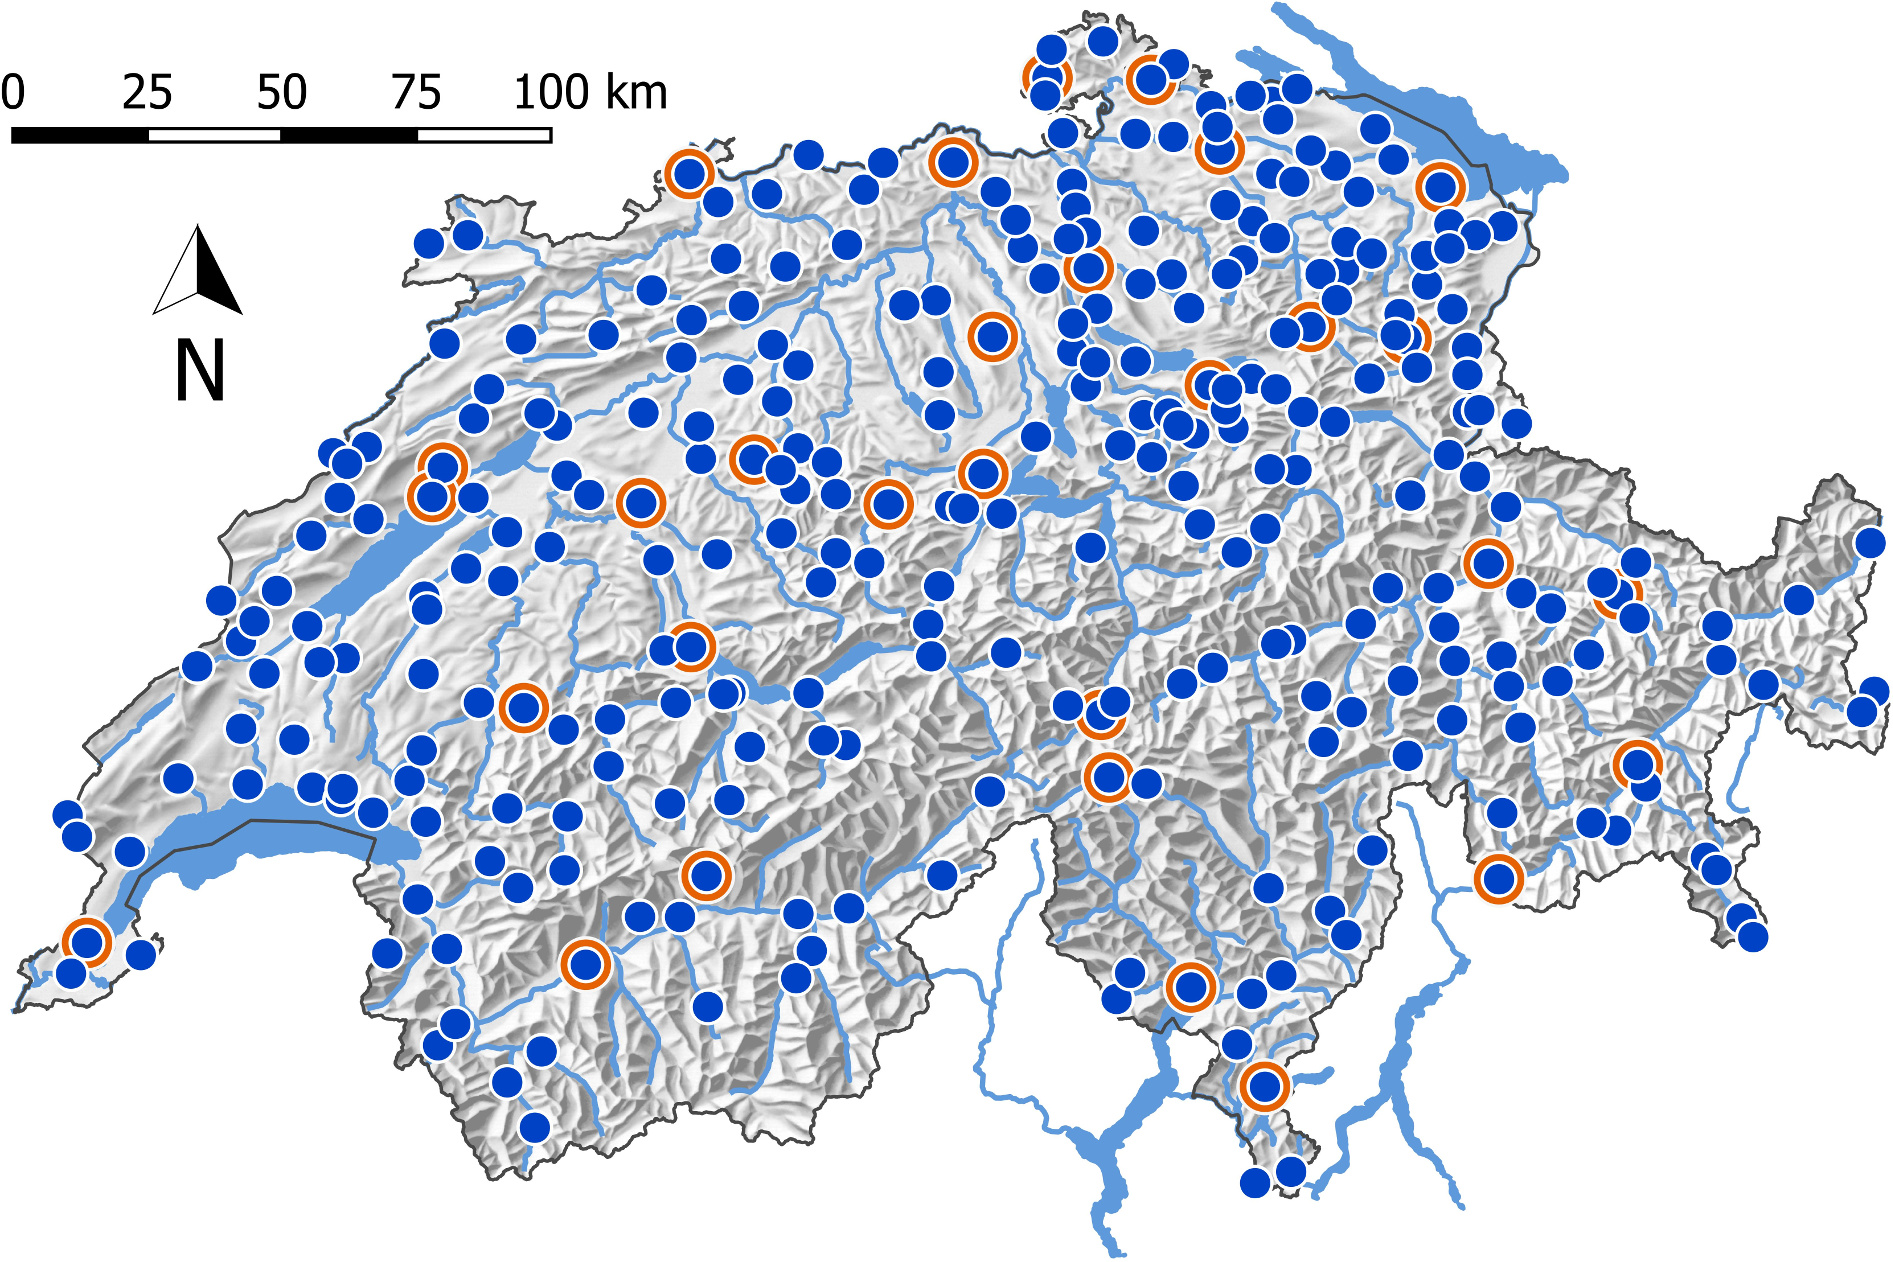
\includegraphics[width=19pc,angle=0]{figure01.pdf}\\
%  \caption{Enter the caption for your figure here.  Repeat as
%  necessary for each of your figures. Figure from \protect\cite{Knutti2008}.}\label{f1}
%\end{figure}

\end{document}